%!TEX root = ../thesis.tex

\section{背景}
近年,工場内の巡回や,警備.また,ラストワンマイル問題の解決に向けた配送業務などで
自律移動ロボットが活用されている.
実世界では,LiDARやGNSSなどのある特定のセンサが機能しない状況に
おちいり.ロボットの自律移動を継続することが困難になる場合がある.
この問題の対処には,複数のセンサを統合して利用する方法や,ロボットに
ナビゲーション手段自体を複数持たせる(冗長化)する方法が考えられる.

ナビゲーション手段の冗長化に向けて,
本研究室の岡田らは,\ref{fig:imi_abs}に示すように
一般的に用いられるLiDARやオドメトリ,
メトリックマップに基づくナビゲーションの行動を
視覚を入力としてend-to-endで模倣学習することで,
視覚に基づくナビゲーションを獲得する手法を提案している.
この手法の特長として,学習のデータセットに利用する行動と
学習時にロボットを制御する行動を別々にして扱うことで
ロボットが経路から外れたときでも,常に経路に戻る行動をデータセットに追加できる.
また実験を通して,視覚に基づいてロボットが学習した経路を周回可能であることが確認した.
岡田らはさらに,訓練時に計測したデータの全てをデータセットに加えるのではなく, 学習器の出力
を監視して, 経路追従できない場所のデータのみ選択してデータセットに追加する手法を追加している.
これにより,目標角速度のデータセットの偏りを減少し,角の経路でも経路を追従できる可能性が向上することが
確認されている.
\begin{figure}[htbp]
     \centering
      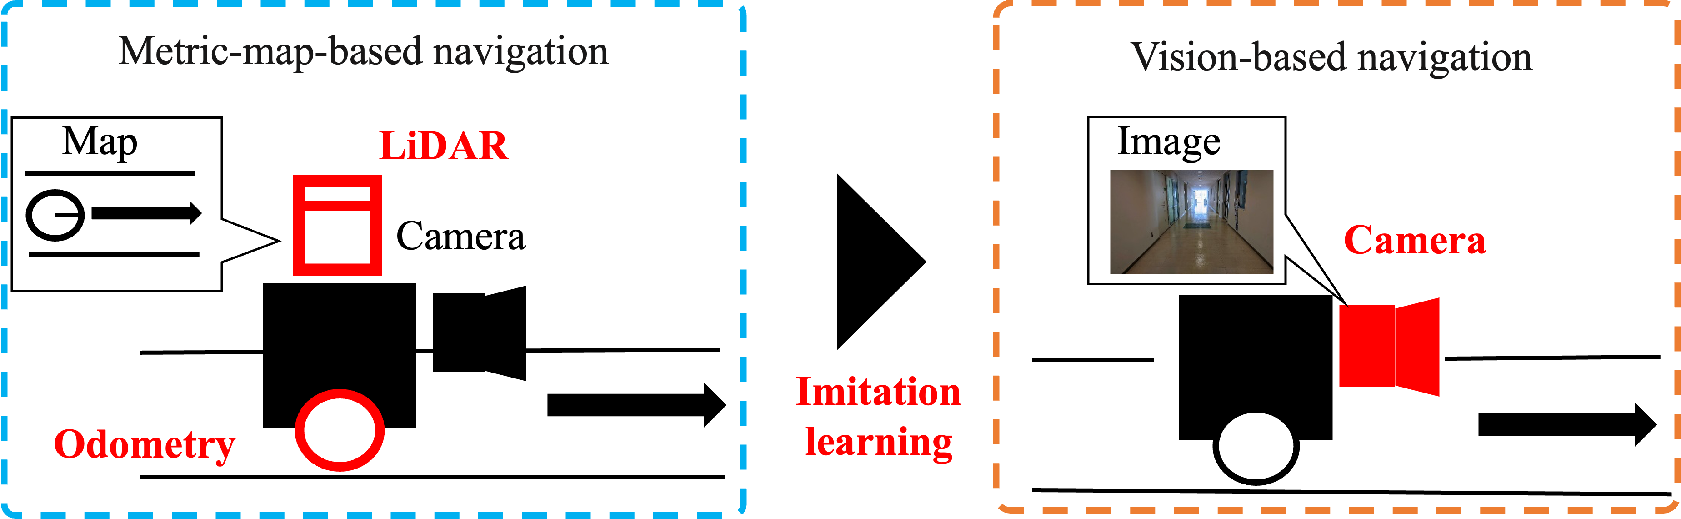
\includegraphics[width=130mm]{images/pdf/imi_abs.pdf}
      \caption{Imitation method of path-tracking behavior}\label{fig:imi_abs}
 \end{figure}

 \begin{figure}[htbp]
     \centering
      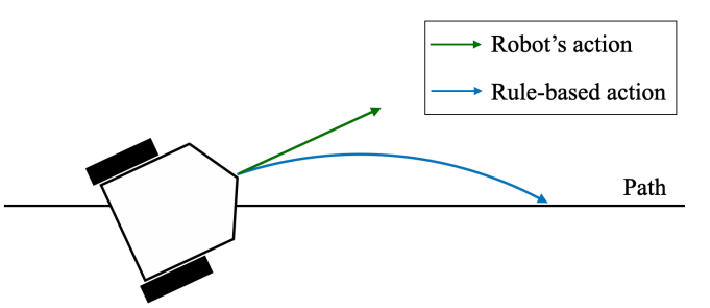
\includegraphics[width=100mm]{images/pdf/robo_action.pdf}
      \caption{Rule-based actions
      apart from the robot's actions Quoted from\cite{okada2020}}
      \label{fig:robo_ac}
 \end{figure}

春山らは,前述の岡田らの手法に対し,
目標とする進行方向の情報(目標方向)を加えることで,
視覚に基づくナビゲーションに分岐路で経路を選択して移動する
機能を追加している.
これにより,ロボットは\ref{fig:haru_select}のように
指示された方向に移動するように,
カメラ画像に基づいて経路を移動する
また,藤原らは,この経路を選択する機能を学習する際に,
オーバーサンプリングや学習時に積極的に蛇行する手法を取り入れることで,
学習時間を短縮する手法を提案している.

 \begin{figure}[htbp]
     \centering
      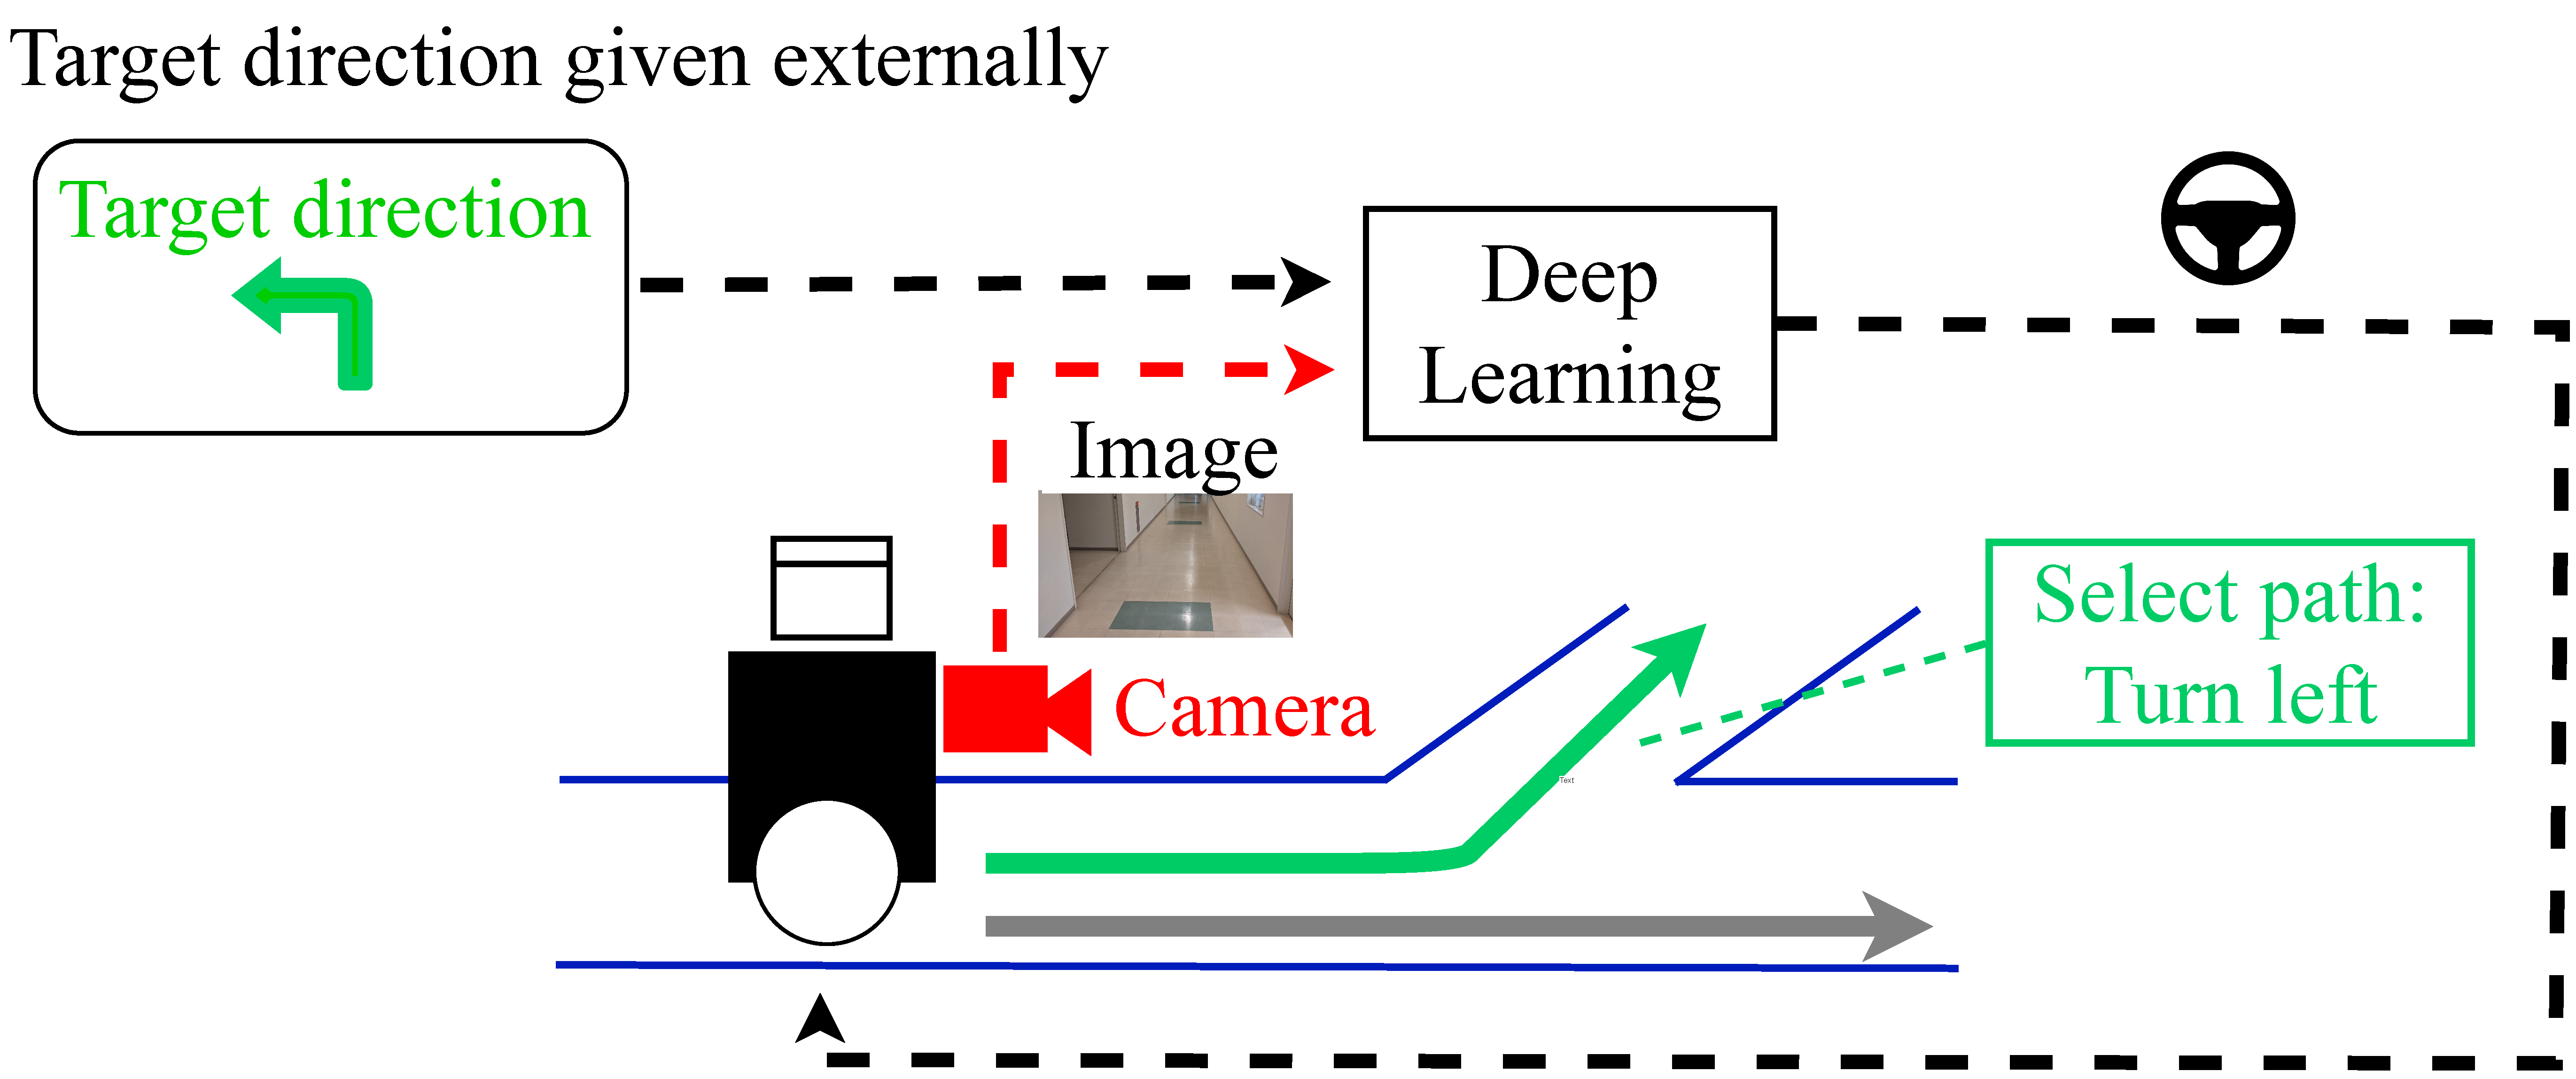
\includegraphics[width=130mm]{images/pdf/learning_gamma.pdf}
      \caption{Path selection and following behavior based 
      on camera images and target direction by imitation learning.}\label{fig:haru_select}
 \end{figure}

春山らと藤原らの手法では,目標方向の
作成方法は議論の対象としておらず,
分岐路における目標方向の生成は,カメラ画像から行っていない.
つまり,視覚のみで目的まで自律移動することは困難となっていた.
そこで,本稿では,視覚のみで目的地まで自律移動するために,
前述の経路を選択する機能をもつ視覚に基づくナビゲーションに対し,
目的の分岐路に到達したかの判定を視覚で行い,目標方向を提示する機能を追加
を追加する.
このシステムにより,事前に作成したメトリックマップを必要せずに,
カメラ画像を入力として目的地まで自律移動できる可能性がある.
\newpage
